% !TeX program = xelatex
\documentclass[11pt]{article}

% Change "review" to "final" to generate the final (sometimes called camera-ready) version.
% Change to "preprint" to generate a non-anonymous version with page numbers.
\usepackage[review]{acl}

% Standard package includes
\usepackage{latexsym}
\usepackage{fontspec}
\setmainfont{TeX Gyre Termes}
\setmonofont{FreeSerif}

% TeX Gyre Termes has no Sinhala coverage, so Sinhala text set in the main font
% renders as missing glyphs. Declare a Sinhala-capable family and wrap every
% Sinhala run in \si{...}. Install a Noto Sinhala font, or change the name to
% one present on the build machine (e.g. "Iskoola Pota" on Windows).
\newfontfamily\sinhalafont{Noto Serif Sinhala}[Script=Sinhala, Scale=0.95]
\newcommand{\si}[1]{{\sinhalafont #1}}

\usepackage{microtype}
\usepackage{graphicx}
\usepackage{booktabs}
\usepackage{multirow}
\usepackage{fvextra}
\DefineVerbatimEnvironment{prompt}{Verbatim}{breaklines=true,breakanywhere=true,fontsize=\small}

% If the title and author information does not fit in the area allocated, uncomment the following
% \setlength\titlebox{5cm}

\title{A Benchmark for AI-Generated Text Detection in Sinhala: \\
Dataset Construction and Preliminary Boundary Detection Results}

\author{
  \textbf{First Author\textsuperscript{1}},
  \textbf{Second Author\textsuperscript{1}},
  \textbf{Third Author\textsuperscript{1}},
  \textbf{Fourth Author\textsuperscript{1}} \\
  \textsuperscript{1}Department of Computer Science and Engineering, University of Moratuwa \\
  \small{\textbf{Correspondence:} \href{mailto:email@domain}{email@domain}}
}

\begin{document}
\maketitle

\begin{abstract}
Large language models can now generate fluent Sinhala text, yet Sinhala, a low-resource language with more than sixteen million speakers, has no public dataset or detector for identifying machine-generated text, while online tools that rewrite such text to evade detection are already available. We present the first benchmark for detecting AI-generated Sinhala text. It comprises a multi-domain parallel corpus for document level human versus machine classification, spanning news, Wikipedia, and social media, and a companion dataset for boundary detection, the task of locating the point in a document where authorship changes from human to machine. Human text is drawn from sources predating the public release of ChatGPT, and each item is paired with machine counterparts from three language models, one of which is held out for cross-model evaluation. We document a reproducible construction pipeline and a cross-model and cross-domain evaluation protocol. On a preliminary slice of the boundary-detection data, a fine-tuned XLM-RoBERTa tagger reaches 0.51 exact-boundary F1, well above position and linear baselines, but its accuracy falls on the held-out generator, and internal rewriting proves substantially harder to detect than continuation. To our knowledge this is the first documented dataset and methodology for detecting AI-generated Sinhala text.
\end{abstract}

\section{Introduction}

The automatic detection of machine-generated text has become an active area of research, as large language models (LLMs) produce increasingly fluent output across many languages \citep{li-etal-2024-mage, wang-etal-2024-m4}. A recurring finding in this literature is that detection generalizes poorly. Detectors trained on a particular set of generators and domains perform substantially worse on unseen ones \citep{wang-etal-2024-m4, wang-etal-2024-m4gt}, and broad multilingual pretraining does not guarantee that a given language is handled reliably \citep{macko-etal-2023-multitude}. Detection capability must therefore be established and measured for each language in turn.

Sinhala has so far fallen outside this effort. Although it is spoken by more than sixteen million people, it remains a low-resource, morphologically rich language with no annotated corpora and no standard tooling for detecting AI-generated text. It is currently unknown whether any detector, whether general-purpose or Sinhala-specific, can reliably separate human-written Sinhala from its machine-generated counterpart. The need is concrete rather than hypothetical, as education, journalism, and social media in Sri Lanka operate substantially in Sinhala, and online tools that rewrite AI-generated Sinhala to evade detection are already publicly available. The closest regional precedent, the DravidianLangTech shared task on Tamil and Malayalam \citep{kodali-etal-2025-bytesizedllm, barua-etal-2025-cuet}, addresses a comparable setting but does not cover Sinhala.

We address this gap by building the first benchmark for detecting AI-generated Sinhala text, and we study two tasks. The first is document-level binary classification, distinguishing human-written from machine-generated text across news, Wikipedia, and social media. The second is boundary detection, locating the sentence at which a document changes from human to machine authorship, which is the harder problem of localizing a stylistic discontinuity inside largely human text. For both tasks we construct parallel data in which human text is paired with machine text from three language models under controlled prompting, adapting the multi-generator and multi-domain design of M4, M4GT-Bench, and MAGE \citep{wang-etal-2024-m4, wang-etal-2024-m4gt, li-etal-2024-mage} to a single low-resource language. We document a reproducible construction pipeline and an evaluation protocol that reports generalization to a held-out generator and a held-out domain rather than a single pooled score. As an initial technical validation, we report preliminary boundary-detection results on a first slice of the corpus. They show that the task is feasible in Sinhala but far from solved, that generalization to an unseen generator is materially harder, and that internal rewriting is much harder to detect than a trailing machine continuation.

The remainder of the paper is organized as follows. Section~\ref{sec:data} describes the construction of both datasets. Section~\ref{sec:binary} presents the binary classification setup, and Section~\ref{sec:boundary} the boundary detection experiments and results. Section~\ref{sec:conclusion} concludes.

\section{Dataset Construction}
\label{sec:data}

Each dataset pairs human-written Sinhala text with machine-generated text on the same content, following the parallel, topic-controlled design of M4 and M4GT-Bench \citep{wang-etal-2024-m4, wang-etal-2024-m4gt}.

\subsection{Human Sources}

Human text is collected from three domains. News is taken from NSINA, a corpus of Sinhala articles from established outlets;\footnote{\url{https://huggingface.co/datasets/sinhala-nlp/NSINA}} Wikipedia from a Sinhala Wikipedia export of 26{,}470 articles;\footnote{\url{https://huggingface.co/datasets/omarkamali/wikipedia-monthly}} and social media from an openly licensed Sinhala Facebook corpus.\footnote{\url{https://huggingface.co/datasets/sinhala-nlp/FacebookDecadeCorpora}} To guarantee human authorship, all source text predates the public release of ChatGPT in November 2022. Following M4, we remove references, URLs, and very short paragraphs, so that the human side does not carry a format-level signal.

\subsection{Binary Detection Data}

For document-level classification, every human item is paired with machine counterparts generated on the same content by three language models: GPT-4o, DeepSeek~V3, and Gemini~2.5~Pro. Two generation modes are used. In \emph{title-to-text} generation, the model writes a full article or answer from only the title or question. In \emph{paraphrase}, the model rewrites the full human text while preserving its facts. News and Wikipedia use both modes; social media, whose posts have no separate title, uses paraphrase only.

All prompts are written natively in Sinhala, since English instructions that merely request Sinhala output tend to induce translationese, which becomes a spurious artifact. To keep detectors from overfitting to a single prompt, each domain and mode uses several prompt variants, a practice shown to improve detector generalization \citep{hao-etal-2025-learning}. Generated length is targeted to a band around the paired human text, so that output length does not become a trivial shortcut. Each source item is assigned to one mode and prompt variant by a fixed-seed allocation, so that the filled prompt for a given item is identical across all three models and their outputs are directly comparable. The target is 500 machine documents per domain and generator, each paired one-to-one with a human document.

\subsection{Boundary Detection Data}

For boundary detection, mixed-authorship documents are constructed from the Wikipedia subset, using the same three generators with Gemini~2.5~Pro held out. After cleaning, long articles are reduced to contiguous windows of six to twelve sentences, and each window is turned into a mixed document by replacing part of it with machine text. Three constructions are used. In \emph{continuation}, a human prefix sampled between 20\% and 80\% of the passage is followed by a machine continuation that replaces the true remainder, giving a single boundary. In \emph{single-span replacement}, one internal span of one to three sentences is rewritten, leaving human text on both sides. In \emph{multi-span replacement}, two or three non-adjacent spans are each rewritten independently from the original human text, which prevents the model from imposing a uniform machine register across the document. Replacement, rather than insertion of invented sentences, keeps the surrounding human text genuine and constrains the machine text to the content it replaces. Every sentence is labelled human or machine, and boundaries are derived from the label sequence.

\subsection{Cleaning, Quality Control, and Splits}

Cleaning is minimal and deterministic, because punctuation, spelling variation, and sentence structure may carry authorship information, and aggressive cleaning can itself introduce class-specific artifacts \citep{wu-etal-2024-detectrl}. Machine preambles, refusals, and markdown are removed, and equivalent rules are applied to the human side, so that neither class carries a format-level tell. Quality control is applied at the model level rather than the example level: a generator producing degenerate Sinhala is dropped in full. On this basis a fourth candidate generator, Mistral~Nemo, was piloted and rejected, as it produced malformed or meaningless Sinhala that nonetheless passed automatic format checks, confirming that those checks gate format rather than fluency.

To prevent topic leakage, all items derived from the same human source are kept in the same partition, so that a detector cannot exploit shared subject matter instead of authorship. Partitions are assigned over source identifiers with a fixed seed and frozen. Two generalization conditions are built in: a held-out generator, Gemini~2.5~Pro, absent from training and development, and a held-out domain, social media, the most stylistically distinct of the three.

\section{Binary Classification}
\label{sec:binary}

\paragraph{Detectors.} We fine-tune four pretrained encoders, all RoBERTa-family so that a single training procedure applies. XLM-R \citep{conneau-etal-2020-unsupervised} is the multilingual baseline, the strongest multilingual encoder covering Sinhala in prior Sinhala text-classification work \citep{dhananjaya-etal-2022-bertifying}. mDeBERTa-v3 \citep{he-etal-2021-debertav3} shares XLM-R's pretraining corpus but uses ELECTRA-style pretraining. SinBERT-small \citep{dhananjaya-etal-2022-bertifying} and SinhalaBERTo \citep{liu-etal-2019-roberta, ortizsuarez-etal-2020-monolingual} are Sinhala-only encoders that separate the effect of in-language pretraining from that of model capacity. We additionally include cheap statistical baselines and off-the-shelf commercial detectors, the latter expected to fail on Sinhala, which is itself a reportable result.

\paragraph{Protocol.} We evaluate under three conditions. \emph{In-distribution} draws train, development, and test from the same generators and domains, using a grouped 70/15/15 split over source groups. \emph{Cross-model} holds out one generator entirely, with Gemini~2.5~Pro as the primary held-out model because it differs most in laboratory, tokenizer, and training mixture. \emph{Cross-domain} holds out social media. The held-out condition is excluded from development as well as training, so that checkpoint selection cannot exploit it. The primary metric is macro-F1, following the DravidianLangTech shared task \citep{kodali-etal-2025-bytesizedllm}; we report the mean over three seeds and break results down by held-out generator and domain, since a pooled score can hide a generalization failure. Table~\ref{tab:binary} reports the in-distribution comparison.

\begin{table}[t]
\centering
\small
\begin{tabular}{lccc}
\toprule
\textbf{Model} & \textbf{Acc.} & \textbf{Macro-F1} & \textbf{AI-F1} \\
\midrule
XLM-R base       & -- & -- & -- \\
mDeBERTa-v3-base & -- & -- & -- \\
SinBERT-small    & -- & -- & -- \\
SinhalaBERTo     & -- & -- & -- \\
\bottomrule
\end{tabular}
\caption{In-distribution binary classification results (mean over three seeds). \textbf{[To be completed once training runs finish.]}}
\label{tab:binary}
\end{table}

\section{Boundary Detection}
\label{sec:boundary}

\paragraph{Task.} Given a document segmented into sentences, the task is to label each sentence as human- or machine-written and thereby locate the boundaries at which authorship changes, where a boundary lies between two adjacent sentences with differing labels. Boundaries are always \emph{derived} from the label sequence rather than stored separately, so generation, assembly, and evaluation share one definition by construction.

\paragraph{Data.} The results below use a preliminary 20\% slice of the planned corpus: 854 documents, 7{,}935 labelled sentences, and 798 source articles, of which 35.8\% of sentences are machine-written. Documents contain 8 to 11 sentences at the quartiles (median 9). Table~\ref{tab:boundary-data} gives the composition. The held-out generator is absent from training by construction, and no source article appears in more than one partition; both invariants are verified on the built dataset.

Construction types are close to balanced: continuation 313 documents (mean 1.00 boundaries, 49.1\% machine sentences), single-span 285 (2.00 boundaries, 24.6\%), and multi-span 256 (5.01 boundaries, 33.2\%). Figure~\ref{fig:positions} shows where boundaries fall.

\paragraph{Setup.} We train on the training split, which contains only the seen generators, and select the model and decision threshold on development data \emph{restricted to seen generators}, so that the held-out generator does not influence model selection. This restriction matters: the held-out generator is present in development as well as test, and tuning on all of development would select hyperparameters using the very generator whose novelty is then reported. We then report on test, overall and separately for seen and held-out generators.

\paragraph{Metrics.} We report exact-boundary F1 as the primary metric, together with F1 on the machine class. Boundaries are matched one-to-one and greedily within a tolerance. We avoid accuracy, because the human class is 64\% of sentences and a human-only predictor reaches 0.644 accuracy while detecting nothing. We also avoid a one-sentence boundary tolerance, since it rewards over-prediction: a random baseline reaches 0.542 under it. Exact-boundary F1 is the only metric the trivial baselines cannot exploit, since predicting a single class everywhere yields no boundaries at all.

\paragraph{Models.} We compare trivial baselines, a position-only baseline that predicts from normalized sentence position with no text, a per-sentence linear classifier over character n-gram features, and a fine-tuned XLM-RoBERTa \citep{conneau-etal-2020-unsupervised} tagger. The position-only baseline bins normalized sentence position and predicts the majority training label of each bin; because boundaries are sampled within a bounded band, it quantifies how much of any score is positional artifact rather than detection. The linear model uses character 3- to 5-grams weighted by sublinear TF-IDF with balanced class weights, chosen over word features because Sinhala is highly inflected and agglutinative; the reported variant also encodes the neighbouring sentences as a second feature block. The tagger encodes the whole document in one pass with a marker token before each sentence, so that each sentence representation is formed with its neighbours in attention range and can express discontinuity rather than an isolated judgement, following the sequence-labelling formulation of \citet{wang-etal-2023-seqxgpt}. Documents longer than the encoder window are chunked on sentence boundaries rather than truncated, so sentence and label sequences always stay aligned; the median document is 335 sub-word tokens and only 3.0\% exceed the 512-token window.

\paragraph{Implementation.} The tagger is \texttt{xlm-roberta-base} fine-tuned for 12 epochs at learning rate $3\times10^{-5}$, batch size 4 without gradient accumulation (1{,}584 optimizer steps), mixed precision, and inverse-frequency class weights. We restore the best epoch by development F1 and tune the decision threshold on development data restricted to seen generators, giving 0.800. Training takes 24.6 minutes on a single 6\,GB consumer GPU, so the experiment is reproducible without cluster resources. We note that an earlier configuration using gradient accumulation gave only 165 optimizer steps, and the model collapsed to the majority class with a loss frozen near $\ln 2$; a 16-document overfitting check reached F1 1.000 and thereby isolated the fault to the optimization schedule rather than the model. We report this because a collapsed tagger yields numbers that closely resemble a genuine negative result about task difficulty.

\paragraph{Results.} Table~\ref{tab:boundary-main} reports the comparison and Figure~\ref{fig:models} visualizes it. The XLM-RoBERTa tagger reaches 0.513 exact-boundary F1 and 0.718 machine-class F1, well above the position-only baseline (0.421) and the best linear model (0.295). Four findings follow.

First, document context is necessary rather than merely helpful. The linear per-sentence classifier scores \emph{below} the position-only baseline on exact boundaries, 0.295 against 0.421, despite higher sentence accuracy, because it can recognize machine-sounding sentences but cannot represent the discontinuity between neighbours. Encoding the document jointly raises exact-boundary F1 to 0.513.

Second, generalization to an unseen generator is materially harder. As Table~\ref{tab:boundary-gen} and Figure~\ref{fig:gap} show, the tagger falls from 0.749 to 0.671 machine-class F1 and from 0.554 to 0.460 exact-boundary F1 between seen and held-out generators, while document-exact accuracy more than halves, from 0.238 to 0.093. This gap is visible only because the held-out generator was excluded from training before generation began.

Third, continuation is far easier to detect than internal rewriting, as Table~\ref{tab:boundary-type} shows. The continuation construction reaches 0.877 machine-class F1, while single-span and multi-span replacement reach 0.588 and 0.592. A trailing machine block is detectable; short rewritten spans embedded in human text are not. The ordering inverts on exact-boundary F1, where continuation is \emph{lowest} at 0.410 against 0.570 for multi-span, because a continuation document offers exactly one boundary and no partial credit, whereas a multi-span document offers up to six.

Fourth, naive structural post-processing hurts. Merging predicted authorship runs shorter than two sentences lowered exact-boundary F1 from 0.295 to 0.201, because multi-span spans are one to two sentences by design and the smoother deletes genuine spans along with noise. Any structural prior over run length must therefore admit single-sentence spans.

These numbers come from a 20\% slice, with development F1 still improving at the end of training while training loss fell to 0.084, and should therefore be read as a lower bound.

\begin{table}[t]
\centering
\small
\begin{tabular}{llrrrr}
\toprule
\textbf{Generator} & \textbf{Role} & \textbf{Train} & \textbf{Dev} & \textbf{Test} & \textbf{All} \\
\midrule
DeepSeek V3    & seen     & 249 & 51 & 52 & 352 \\
GPT-4o         & seen     & 253 & 59 & 53 & 365 \\
Gemini 2.5 Pro & held-out & 0   & 62 & 75 & 137 \\
\midrule
\textbf{Total} &          & \textbf{502} & \textbf{172} & \textbf{180} & \textbf{854} \\
\bottomrule
\end{tabular}
\caption{Boundary-detection data (20\% slice), in documents. The held-out generator writes only development and test.}
\label{tab:boundary-data}
\end{table}

\begin{table}[t]
\centering
\small
\setlength{\tabcolsep}{4pt}
\begin{tabular}{lccccc}
\toprule
& \multicolumn{3}{c}{\textbf{Sentence}} & \multicolumn{2}{c}{\textbf{Boundary}} \\
\cmidrule(lr){2-4}\cmidrule(lr){5-6}
\textbf{Model} & \textbf{Acc.} & \textbf{F1} & \textbf{P} & \textbf{exact} & \textbf{$\pm$1} \\
\midrule
All human       & 0.644 & 0.000 & 0.000 & 0.000 & 0.000 \\
All AI          & 0.356 & 0.526 & 0.356 & 0.000 & 0.000 \\
Random          & 0.552 & 0.371 & 0.371 & 0.360 & 0.542 \\
Position only   & 0.686 & 0.518 & 0.571 & 0.421 & 0.612 \\
Linear (best)   & 0.720 & 0.586 & 0.619 & 0.295 & 0.508 \\
\textbf{XLM-R}  & \textbf{0.790} & \textbf{0.718} & \textbf{0.690} & \textbf{0.513} & \textbf{0.702} \\
\bottomrule
\end{tabular}
\caption{Boundary detection on the test set (20\% slice). Sentence F1 and precision are for the machine class. Exact-boundary F1 is the metric the trivial baselines cannot game; the $\pm$1 column is shown only to justify excluding it, since Random reaches 0.542 under it.}
\label{tab:boundary-main}
\end{table}

\begin{table}[t]
\centering
\small
\setlength{\tabcolsep}{4pt}
\begin{tabular}{llccc}
\toprule
\textbf{Test slice} & \textbf{Role} & \textbf{Sent.\ F1} & \textbf{Bound.} & \textbf{Doc.} \\
\midrule
DeepSeek V3    & seen     & 0.761 & 0.562 & -- \\
GPT-4o         & seen     & 0.736 & 0.547 & -- \\
Gemini 2.5 Pro & held-out & 0.671 & 0.460 & -- \\
\midrule
All seen       & seen     & 0.749 & 0.554 & 0.238 \\
Held-out       & held-out & 0.671 & 0.460 & 0.093 \\
\bottomrule
\end{tabular}
\caption{XLM-R by generator. \textbf{Bound.} is exact-boundary F1 and \textbf{Doc.} the fraction of documents whose entire boundary set is predicted exactly. The seen/held-out gap is the paper's central generalization result.}
\label{tab:boundary-gen}
\end{table}

\begin{table}[t]
\centering
\small
\setlength{\tabcolsep}{4pt}
\begin{tabular}{lcccc}
\toprule
& \multicolumn{2}{c}{\textbf{Sent.\ F1}} & \multicolumn{2}{c}{\textbf{Bound.\ exact}} \\
\cmidrule(lr){2-3}\cmidrule(lr){4-5}
\textbf{Construction} & \textbf{Lin.} & \textbf{XLM-R} & \textbf{Lin.} & \textbf{XLM-R} \\
\midrule
Continuation        & 0.787 & \textbf{0.877} & 0.262 & \textbf{0.410} \\
Single-span replace & 0.357 & \textbf{0.588} & 0.226 & \textbf{0.493} \\
Multi-span replace  & 0.346 & \textbf{0.592} & 0.152 & \textbf{0.570} \\
\bottomrule
\end{tabular}
\caption{Results by construction type. Continuation is far easier than embedded rewriting on sentence F1, but the ordering inverts on exact-boundary F1, where a single-boundary document allows no partial credit.}
\label{tab:boundary-type}
\end{table}

\begin{figure*}[t]
\centering
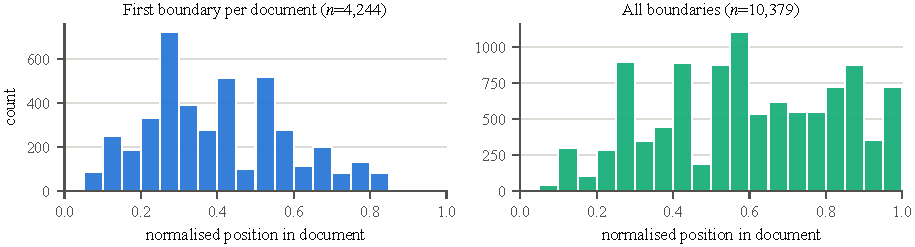
\includegraphics[width=\textwidth]{figures/fig1_boundary_positions.pdf}
\caption{Normalized boundary positions in the boundary-detection data. The distribution is spread rather than spiked, with only 2.1\% of first boundaries in the leading tenth of a document, but it is not uniform: the 20--80\% sampling rule and the constraint that spans may not include the first sentence together produce a band. This is the prior the position-only baseline exploits, and the reason it is reported. Mass at 1.0 in the right panel is legitimate, arising when a span ends immediately before the final sentence.}
\label{fig:positions}
\end{figure*}

\begin{figure*}[t]
\centering
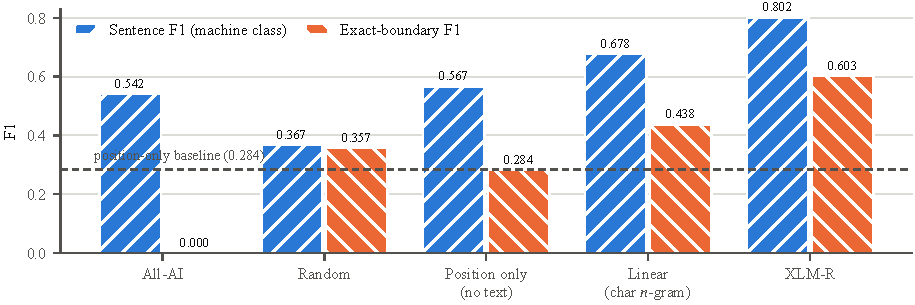
\includegraphics[width=\textwidth]{figures/fig2_model_comparison.pdf}
\caption{Boundary detection on the test set. The dashed line marks the position-only baseline, which reads no text at all. The linear per-sentence classifier falls below it on exact-boundary F1 despite the higher sentence F1, showing that recognizing machine-sounding sentences is not the same as localizing authorship change; only the document-level tagger clears the line.}
\label{fig:models}
\end{figure*}

\begin{figure*}[t]
\centering
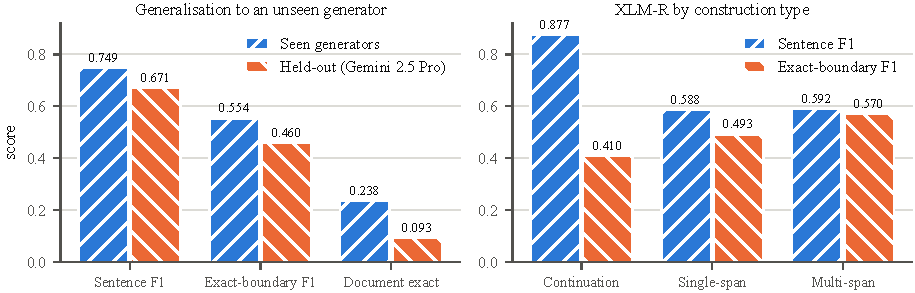
\includegraphics[width=\textwidth]{figures/fig3_generalisation_and_type.pdf}
\caption{Left: XLM-R on seen versus held-out generators. The gap widens as the metric becomes stricter, and document-exact accuracy more than halves. Right: XLM-R by construction type. Continuation has the highest sentence F1 but the lowest exact-boundary F1, since it offers a single boundary and no partial credit.}
\label{fig:gap}
\end{figure*}

\section{Conclusion and Future Work}
\label{sec:conclusion}

We have presented the first benchmark for detecting AI-generated Sinhala text, comprising a multi-domain parallel corpus for binary classification and a companion boundary-detection dataset, together with a reproducible construction pipeline and a cross-model, cross-domain evaluation protocol. Preliminary boundary-detection results show the task is feasible but unsolved, that generalization to an unseen generator is markedly harder, and that internal rewriting resists detection far more than continuation. Future work will complete generation across the full corpus, run the binary detector suite, add a second held-out generator of a different family, and extend boundary detection beyond the encyclopedic domain. The dataset, code, and evaluation harness will be released as a reference resource.

\section*{Limitations}

Results are from a preliminary 20\% slice of the boundary-detection corpus, so the transformer numbers are a lower bound, and the binary detectors are not yet evaluated. Generalization is measured against a single held-out generator, which cannot separate generalization to unseen models in general from generalization to one model in particular. Boundary detection covers only the encyclopedic register of Wikipedia, whose human text carries typographic noise that clean machine text lacks, so a detector may partly learn that cleaner text is machine-written; this confound is not yet controlled. By construction, boundaries fall between the first and last sentences and within a bounded length band, which a position-only baseline partly exploits. Finally, no human annotation study establishes the ceiling for either task, so it is not known how close the reported scores are to the achievable maximum.

\section*{Ethics Statement}

This work supports the detection of AI-generated text and does not develop or promote evasion methods. All human text is drawn from publicly available, openly licensed corpora that predate widespread LLM use. The benchmark is intended to help educators, journalists, and platform moderators verify the origin of Sinhala content, and it will be released for research use.

\bibliography{custom}

\appendix
\input{prompt_templates}
\section{Boundary-Detection Examples}
\label{app:boundary-examples}

Three documents from the boundary-detection data, one per construction type,
shown with their gold sentence labels. Sentences are numbered as in the record;
\textbf{M} marks a machine-written sentence and H a human one. Sinhala is
reproduced verbatim, including the orthographic noise present in the source
articles.

\subsection{Continuation (single boundary)}

Article \si{මැඩගස්කරයේ භූගෝලය} (\emph{Geography of Madagascar}), generated by
DeepSeek~V3. Labels $[0,0,0,0,1,1]$, one boundary before sentence~4. The human
remainder was discarded and replaced by a machine continuation of matched
length.

\begin{table}[h]
\centering
\small
\begin{tabular}{@{}cl p{0.80\columnwidth}@{}}
\toprule
\# & & Sentence \\
\midrule
0 & H & \si{මිනිසුන් මැඩගස්කරයට පැමිණීමෙන් පසු අවම වශයෙන් ලීමර් විශේෂ 17 ක් වඳ වී ගොස් ඇති අතර, ඒවා සියල්ලම ඉතිරිව ඇති ලීමර් විශේෂයට වඩා විශාල විය.} \\[2pt]
1 & H & \si{ෆොසා (බළලුන් වැනි) ඇතුළු තවත් ක්ෂීරපායින් ගණනාවක් මැඩගස්කරයට ආවේණික වේ.} \\[2pt]
2 & H & \si{දිවයිනේ කුරුලු විශේෂ 300කට අධික ප්‍රමාණයක් වාර්තා වී ඇති අතර ඉන් සියයට 60කට වැඩි ප්‍රමාණයක් ආවේණික වේ.} \\[2pt]
3 & H & \si{(එක් ආවේණික පවුලක් ඇතුළුව).} \\[2pt]
4 & \textbf{M} & \si{මැඩගස්කරයේ සීනීන් ඇතුළුව උභයජීවීන්ගේ විශේෂ 370කට අධික ප්‍රමාණයක් වාර්තා වී ඇති අතර ඉන් සියයට 99කට වැඩි ප්‍රමාණයක් ආවේණික වේ.} \\[2pt]
5 & \textbf{M} & \si{තවද මෙම දිවයිනේ කටුස්සා වැනි සත්ව විශේෂ ගණනාවක් පමණක් නොව සත්ව ගණයේ අනන්‍යතාවයන් දක්නට ලැබේ.} \\
\bottomrule
\end{tabular}
\end{table}

The boundary is not lexically marked. Sentence~4 continues the endemism
statistics of sentence~2 in the same register and with the same construction,
which is the intended difficulty.

\subsection{Single-span replacement}

Article \si{රෙකෝන්ඩය} (\emph{Recorder}), generated by GPT-4o. Labels
$[0,0,0,1,0,0]$, two boundaries, with one internal sentence rewritten and human
text on both sides.

\begin{table}[h]
\centering
\small
\begin{tabular}{@{}cl p{0.80\columnwidth}@{}}
\toprule
\# & & Sentence \\
\midrule
2 & H & \si{මෙය දැවය භාණ්යක් වන අතර ඇගිලි ගණනක් සදහා සිදුරු සහිත මෙය මුඛ්‍ය හා සම්බන්ධ මත ස්ථානයේ වඩා පලල්වද ඉතා දුරට යන්නට සිහින්මය යන ආකාරයද නිපදවා ඇත.} \\[2pt]
3 & \textbf{M} & \si{මධ්‍ය යුගයේ විශේෂයෙන්ම ජනප්‍රිය වූ රෙකෝඩරය, දහ අටවන ශතවර්ෂයෙන් පසු සංගීත උපකරණයකි, නමුත් ඊට පසුව එහි භාවිතය සන්සුන් වශයෙන් අඩු විය.} \\[2pt]
4 & H & \si{මධ්‍යතන යුගයේ මෙම සංගීත භාණ්ය කොතරම් ජනප්‍රියව කිබණේද යත් සාහිත්‍යමය කලා නිර්මාණ ආදියේ නිර්තන්තර එම සංගීත භාණ්ඩය පිළිබද සටහන් දැකිය හැකි විය.} \\
\bottomrule
\end{tabular}
\end{table}

This example illustrates the confound noted in the Limitations. The machine
sentence is better formed than the human sentences surrounding it, which
contain orthographic errors (\si{භාණ්යක්}, \si{කිබණේද}). A detector may
therefore partly learn that cleaner text is machine-written, which is a
property of the source corpus rather than of the generators.

\subsection{Multi-span replacement}

Article \si{උගන්ඩාවේ භූගෝලය} (\emph{Geography of Uganda}), generated by
DeepSeek~V3. Labels $[0,0,1,0,1,0,1,0]$, six boundaries from three
single-sentence spans, each generated independently from the original human
document.

\begin{table}[h]
\centering
\small
\begin{tabular}{@{}cl p{0.80\columnwidth}@{}}
\toprule
\# & & Sentence \\
\midrule
1 & H & \si{රට සාමාන්‍යයෙන් මුහුදු මට්ටමේ සිට මීටර් 900 ක උසකින් පිහිටා ඇත.} \\[2pt]
2 & \textbf{M} & \si{උගන්ඩාවේ නැගෙනහිර හා බටහිර දෙපසම කඳුකරයන් පිහිටා ඇත.} \\[2pt]
3 & H & \si{රුවෙන්සෝරි කඳුවැටිය උගන්ඩාවේ උසම කඳු මුදුන අඩංගු වන අතර එය ඇලෙක්සැන්ඩ්‍රා ලෙස නම් කර ඇති අතර එහි විශාලත්වය මීටර් 5,094 කි.} \\[2pt]
4 & \textbf{M} & \si{රටේ දකුණු කොටසෙහි විශාල ප්‍රදේශයක් ලෝකයේ විශාලතම විල් ලෙස සැලකෙන වික්ටෝරියා විලේ බලපෑමට යටත්ව ඇති අතර එහි බොහෝ දූපත් දක්නට ලැබේ.} \\[2pt]
5 & H & \si{කම්පාලා අගනුවර සහ එන්ටෙබේ අගනුවර ඇතුළුව මෙම වැව ආසන්නයේ වඩාත් වැදගත් නගර දකුණේ පිහිටා ඇත.} \\[2pt]
6 & \textbf{M} & \si{රටේ මධ්‍යයේ පිහිටි කියෝගා විල පුළුල් වගුරු බිම් වලින් යුක්ත වේ.} \\[2pt]
7 & H & \si{ගොඩබිම් සහිත වුවද උගන්ඩාවේ විශාල විල් රාශියක් ඇත.} \\
\bottomrule
\end{tabular}
\end{table}

Alternating single-sentence spans are the hardest configuration in the dataset.
They are also why run-length smoothing degrades performance: a post-process
that merges authorship runs shorter than two sentences removes every span in
this document.


\end{document}
